\documentclass[11pt,a4paper]{article} 

% Define page geometry
\usepackage{geometry}
\geometry{left=2.2cm,
	right=2.2cm,
	top=2.2cm,
	bottom=2cm} % Page margins
\parskip 0.15cm % Paragraph spacing
\setlength{\parindent}{0cm} % No paragraph indenting

% Text formatting
\usepackage[T1]{fontenc} % Set font
\usepackage{lineno} % Line numbers
\linespread{1.5} % Linespacing

\usepackage{amssymb}
\usepackage{multirow}
\setlength{\tabcolsep}{4pt} % Default table column sep width 

\usepackage{fmtcount}

\usepackage{pdflscape}

\usepackage{longtable}
\setlength{\LTcapwidth}{\textwidth}
\usepackage{booktabs}  % Sensible horizontal rules
\usepackage{array}  % Extended column formats
\usepackage{multirow}  % Tables with cells split over multiple rows
\usepackage{makecell}  % Multi-row table headers


% Image handling
\usepackage{graphicx} 
\graphicspath{ {img/} } % Define image path
\usepackage{float} % Precise figure location

% Bibliography management
\usepackage[natbib, 
	style=authoryear, 
	uniquename=false, 
	uniquelist=false,
	giveninits=true,
	dashed=false,
	maxcitenames=2, 
	mincitenames=1, 
	minbibnames=10, 
	maxbibnames=10, 
	backend=biber]{biblatex}
\renewcommand*\finalnamedelim{\addspace\&\space}
\addbibresource{phenology.bib}

% Links within document, nice figure formatting
\usepackage{xcolor}
\newcommand{\todo}[1]{\textcolor{red}{\textbf{#1}}}   % \todo{NOTE IN RED}
\usepackage[breaklinks]{hyperref}
\definecolor{links}{RGB}{0,0,0}
\hypersetup{
	breaklinks,
	colorlinks=true,
	linkcolor=links,
	anchorcolor=links,
	citecolor=links,
	filecolor=links,
	menucolor=links,
	runcolor=links,
	urlcolor=links,
	pdfauthor={John L. Godlee}
}
\def\subsectionautorefname{section}
\def\subsubsectionautorefname{section}

\newcommand{\beginsupplement}{%
	\setcounter{table}{0}
	\renewcommand{\thetable}{S\arabic{table}}%
	\setcounter{figure}{0}
	\renewcommand{\thefigure}{S\arabic{figure}}%
	}

\usepackage{makecell}

% \DeclareUnicodeCharacter{0301}{*************************************}
   
% Variables
\input{out/vars.tex}

\begin{document}

{\Large{Title: Tree species diversity and structure mediate land surface phenology in seasonally dry tropical woodlands}}

Authors: Godlee J. L.\textsuperscript{1}, Ryan C. M.\textsuperscript{1}, Siampale A.\textsuperscript{2}, Dexter K. G.\textsuperscript{1,3}

\textsuperscript{1}School of GeoSciences, University of Edinburgh, Edinburgh, EH9 3FF, United Kingdom \\
\textsuperscript{2}Forestry Department Headquarters - Ministry of Lands and Natural Resources, Cairo Road, Lusaka, Zambia \\
\textsuperscript{3}Royal Botanic Garden Edinburgh, Edinburgh, EH3 5LR, United Kingdom \\

\vspace{1em}
Corresponding author:

John L. Godlee

johngodlee@gmail.com

School of GeoSciences, University of Edinburgh, Edinburgh, United Kingdom

\section*{Acknowledgements}

\section*{Author contribution statement}

JLG conceived the study, conducted the analysis, and wrote the first draft of the manuscript. AS coordinated plot data collection in Zambia. All authors contributed to manuscript revisions. 

\section*{Data accessibility statement}

The data used in this study are from the Zambian Integrated Land Use Assessment (ILUA-II). Data were cleaned and archived by the SEOSAW project (Socio-Ecological Observatory for Studying African Woodlands). An anonymised version of the plot data are available at the following DOI: \todo{URL for Edinburgh Datashare}. Code developed for data analysis can be found here: \url{https://github.com/johngodlee/zambia_phenology}.

\newpage{}
\linenumbers

\section*{Abstract}

\begin{enumerate}
	\item{Seasonal foliage production (leaf phenology) is a key determinant of
		ecosystem function. Land surface phenology observed via space-borne
		remote sensing, can be predicted to some extent from climate, but we lack
		understanding of how vegetation structure and composition mediates patterns of
		land surface phenology. This hampers our ability to predict phenological
		changes and therefore ecosystem function, in light of rapid ongoing shifts in
		biodiversity and ecosystem structure.}
		
	\item{We combined a dense network of \nSites{} vegetation monitoring sites
		across deciduous woodlands in Zambia with land surface phenology
		metrics to investigate the role of tree species diversity, composition, and
		vegetation structure on patterns of land surface phenology, including the
		phenomenon of pre-rain green-up.} 

	\item{Tree species diversity was associated with earlier pre-rain green-up,
		a longer growing season, and greater cumulative foliage production,
		across all woodland types identified in the study. Proportional abundance
		of Detarioideae species (subfamily of Fabaceae) drive a longer period of
		maximum foliage production by facilitating earlier pre-rain green-up. Woodland
		compositional types differed maginally in their land surface phenology. Larger
		trees can access deep groundwater reserves, facilitating earlier pre-rain
		green-up. Senescence metrics showed consistent variation among sites, but were
		not well explained by any measured variable.}

	\item{This study underlines the importance of vegetation composition,
		diversity and structure as determinants of ecosystem function, and
		offers new insights into the factors determining patterns of land surface
		phenology across the dry tropics, which are essential for realistic modelling
		of land-atmosphere mass and energy exchange.}

	\item{\textbf{Synthesis:} Tree species composition and diversity influence
		seasonal foliage production in deciduous tropical woodlands. More
		diverse woodlands are able to green-up earlier with respect to seasonal
		rains. Detarioideae species (subfamily of Fabaceae), are associated with longer
		growing seasons, effectively extending the period of maximum foliage production
		by facilitating pre-rain green-up. Understanding variation in land surface
		phenology with respect to vegetation composition is of great importance for
		earth-system modellers aiming to parameterise the next generation of predictive
		models of land-atmosphere mass and energy exchange.}
\end{enumerate}

\newpage{}

\section{Introduction}

Foliage forms the primary interface between the vegetated land surface, the
atmosphere and incoming solar radiation \citep{Gu2003, Penuelas2009}. Seasonal
cycles of foliage production (leaf phenology) play an important role in
regulating global carbon, water and nitrogen cycles \citep{Richardson2013}.
Terrestrial biosphere models routinely incorporate vegetation indices derived
from remote sensing products as a proxy for foliage production (land surface
phenology), to constrain estimates of Gross Primary Productivity (GPP)
(\citealt{Bloom2016, Helman2018}). Previous studies have described
environmental drivers of land surface phenology \citep{Adole2019, Guan2014},
but understanding of how the composition and structure of the vegetation itself
affects patterns of land surface phenology is lacking \citep{Whitley2017}. 

At continental scales, land surface phenology can be predicted adequately using
only climatic factors, namely precipitation, diurnal temperature oscillation,
and photoperiod \citep{Adole2018a, Adole2019, Guan2014}, but significant local
variation exists within biomes in the timing of foliage production that cannot
be attributed solely to abiotic environment \citep{Stockli2011}. It has been
repeatedly suggested that the diversity, composition, and structure of plant
communities plays a role in determining ecosystem response to abiotic cues
driving patterns of land surface phenology \citep{Adole2018b, Jeganathan2014,
Fuller1999}, owing to differences in phenological strategy among species.
Indeed, ground observations find wide variation in phenological patterns of
foliage production among plant communities within a given biome
\citep{Seyednasrollah2019}, but this is rarely represented in predictive models
of biosphere-atmosphere exchanges \citep{Scheiter2013, Pavlick2013}.

Across the dry tropics, seasonal oscillations in water availability drive
seasonal cycles of foliage production \citep{Chidumayo2001, Dahlin2016}. The
phenomenon of pre-rain green-up seen in some tree species within the dry
tropics serves as a striking example of adaptation to seasonal variation in
water availability \citep{Ryan2017}. Conservative species, slower growing with
robust leaves and denser wood, may initiate foliage production (green-up)
before the rainy season has commenced. They may also retain their leaves for
longer after the end of the rainy season, though the mechanisms of this
behaviour are less clear \citep{Giraldo2011, Kushwaha2011}. Acquisitive species
however, may only begin to produce foliage during the rainy season, creating a
dense leaf-flush during the mid-season peak of growth and dropping their leaves
earlier as soil water content drops towards the end of the rainy season
\citep{Lasky2016}. While conservative species gain a competitive advantage from
having fully emerged leaves once the rainy season starts, they must also invest
heavily in deep root architecture to access groundwater reserves in order to
produce foliage during the dry season, and risk hydraulic failure if seasonal
rains occur much later than normal \citep{Vinya2018}. It has been suggested
that variation in phenological strategy among tree species is one mechanism by
which increased species diversity increases resilience to drought and maximises
productivity in water-limited woodland ecosystems \citep{Stan2019,
Morellato2016}. 

Variation in seasonal patterns of foliage production affects broader ecosystem
processes. Woodlands with a longer tree growth period support a greater
diversity and abundance of wildlife, particularly birds, but also browsing
mammals and invertebrates \citep{Cole2015, Araujo2017, Morellato2016,
Ogutu2013}. As climate change increases the frequency and severity of droughts
in water-limited woodlands, woodlands with a diverse tree community may provide
refugia for many animal species \citep{Bale2002}. The period of green-up is a
key time for invertebrate reproduction \citep{Prather2012} and herbivore
browsing activity \citep{Velasque2016, Morellato2016}. Pre-rain green-up
provides a valuable source of moisture and nutrients before the rainy season,
and can moderate the understorey microclimate, increasing humidity, reducing UV
exposure, moderating diurnal oscillations in temperature, and reducing
ecophysiological stress which otherwise can lead to mortality during the dry
season. Thus, understanding what drives variation in seasonal patterns of
foliage production in tropical deciduous woodlands can provide valuable
information on their vulnerability to climate change, and therefore better
information to predict their future extent and productivity.

In the miombo woodlands of southern Africa, the largest woodland type in the
region \citep{White1983}, Detarioideae species (subfamily of Fabaceae) are one
such group which exhibit pre-rain green-up. Detarioideae species are frequently
dominant in miombo woodlands, producing tall woodland canopies with deep root
systems \citep{Zhou2020}. Previous studies have shown local variation in land
surface phenology, particularly the pre-rain green-up phenomenon, which is not
explained by climate \citep{Zhou2020}.

In this study we investigate how tree species diversity, composition, and
structure influence land surface phenology in seasonally dry tropical
woodlands. We focus specifically on the lag between green-up/senescence and the
onset/end of the rainy season, the magnitude of foliage production within the
growing season, and the overall length of the growing season. We hypothesise
that: (H\textsubscript{1}) sites with greater species diversity will exhibit a
longer growing season due to a higher diversity of phenological strategies;
(H\textsubscript{2}) in sites with greater species diversity the start of the
growing season will occur earlier with respect to the onset of the rainy season
due to an increased likelihood of containing species which can green-up early;
(H\textsubscript{3}) sites with larger trees will exhibit longer growing
seasons, as large trees can better access deep groundwater reserves outside of
the rainy season; (H\textsubscript{4}) sites dominated by Detarioideae species
will experience earlier pre-rain green-up. 

\section{Materials and Methods}

\subsection{Plot data}

We used data on tree species diversity and composition from \nSites{} sites
surveyed as part of the Zambian Integrated Land Use Assessment Phase II
(ILUA-II), conducted in \censusDate{} \citep{Mukosha2009, Pelletier2018}. Each
site consisted of four 20$\times$50 m (0.1 ha) plots positioned in a
500$\times$500 m square around a central point (\autoref{schematic}), resulting
in a total plot area per site of 4000 m\textsuperscript{2}. The original census
contained \nTotalSites{} sites, which was filtered in order to define study
bounds and to ensure data quality. Only sites with $\geq$\treesHa{} stems
ha\textsuperscript{-1} $\geq$\stemSize{} cm DBH (Diameter at Breast Height)
were included in the analysis, to ensure all sites represented woodlands with a
relatively continuous canopy rather than `grassy savanna', which is considered
a separate biome with different species composition and ecosystem processes
governing phenology \citep{Parr2014}. 

Plots in the ILUA-II dataset sampled stems $\geq$\stemSize{} cm DBH across the
area of the whole plot, while stems <\stemSize{} cm DBH were measured in
10$\times$20 m (0.02 ha) nested subplots. We chose to use only stem
measurements $\geq$\stemSize{} cm DBH in this study, discarding measurements
from the nested subplots. In woodland ecosystems with a relatively continuous
canopy like those studied here, only the larger trees form the canopy layer,
with smaller trees existing within the understorey layer \citep{Chidumayo2001}.
The signal from remotely-sensed measurements of land surface phenology is
dominated by these larger trees which form the woodland canopy. We therefore
reasoned that small stems would not be an important factor in determining
measurements of land surface phenology. To further demonstrate the dominance of
larger stems in our sites, we compared the total basal area contribution of
stems $\geq$\stemSize{} cm with that of stems <\stemSize{} cm DBH, with the
values of the small stems multiplied up to the area of the whole site. We found
that across all sites, the minimum proportional basal area contributed by stems
$\geq$\stemSize{} was \minPropBABig{}\%, while the median was
\medianPropBABig{}\%.

Sites with non-native tree species, e.g. \textit{Pinus} spp. and
\textit{Eucalyptus} spp. were excluded, as these species may exhibit patterns
of foliage production which differ markedly from that of native tree species
assemblages \citep{Broadhead2003}. Of the \nTrees{} trees recorded,
\perSpID{}\% were identified to species. Sites with >20\% of trees not
identified to species were discarded.

\begin{figure}[H]
\centering
	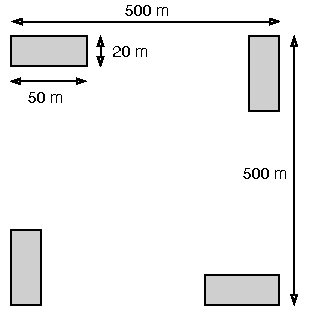
\includegraphics[width=0.5\textwidth]{schematic}
	\caption{Schematic diagram of plot layout within a site. Each 20$\times$50
		m (0.1 ha) plot is shaded grey. Note that the plot dimensions are not to
		scale.}
	\label{schematic}
\end{figure}

Within each plot, the species and basal area of all trees with at least one
stem $\geq$\stemSize{} cm DBH were recorded. Plot data were aggregated to the
site level for analyses to avoid pseudo-replication. Each site spans an area
500$\times$500 m (0.25 km\textsuperscript{2}), matching that of the land
surface phenology data used. We excluded sites where plots differed appreciably
in vegetation composition, to ensure that all sites used in statistical
analysis were representative of the vegetation within the total 0.25
km\textsuperscript{2} area of each site. Using the Bray-Curtis dissimilarity
index on species basal area data \citep{Faith1987}, we calculated the mean
pairwise compositional distance between plots within each site. Sites were
discarded when the mean pairwise compositional distance among plots within the
site was greater than the mean pairwise compositional distance of all plots
across all sites. This resulted in a final dataset of \plotDistN{} sites.

\subsection{Vegetation composition and diversity} 

To classify variation in tree species composition we used agglomerative
hierarchical clustering on species basal area data \citep{Kreft2010,
Fayolle2014}. We excluded species with fewer than five records across all sites
from this analysis, as very rare species can hinder meaningful cluster
delineation. We used Ward's algorithm to define clusters \citep{Murtagh2014},
based on the Bray-Curtis distance between pairs of sites. We determined the
optimal number of clusters by maximising the mean silhouette width among
clusters \citep{Rousseeuw1987}. We described the vegetation types represented
by each cluster using Dufr\^{e}ne-Legendre indicator species analysis
\citep{Dufrene1997}, which ranks species as the product of their relative
frequency and their relative average abundance in each vegetation type.
\Numberstringnum{\nCluster} vegetation types were identified during
hierarchical clustering. The mean silhouette value of the clustering algorithm
reached \silBest{}. 

There was some spatial and climatic stratification in vegetation type
distribution (\autoref{site_map}). Three miombo woodland types were identified,
each with different sets of secondary species, but all dominated by
Detarioideae species such as \textit{Brachystegia} spp. and
\textit{Julbernardia} spp. (\autoref{clust_summ}). Uapaca miombo is largely
absent from the southwest of the country, occurring predominantly in higher
rainfall regions to the north and east (\autoref{box_facet_map_mat}).
Cryptosepalum miombo is found more in the southwest of the country, possibly
representing the drier ``Angolan miombo woodlands'' described by
\citet{White1983}. Importantly, we do not think these woodlands represent the
very different Zambezian evergreen forests, which are dominated by
Cryptosepalum. Julbernardia miombo is common in cooler areas and is more
climatically restricted than the other miombo woodland types. Combretaceae
woodlands match the description of small stature Zambesian woodlands, as
described by \citet{Dinerstein2017} and \citet{Chidumayo2001}. These woodlands
are not dominated by the same archetypal Detarioideae tree species as the other
miombo woodland vegetation types. These Combretaceae woodlands occur over a
wide climatic range, and contain some of the warmest sites in our dataset in
the southeast of the country. The miombo woodland vegetation types are
dominated by \textit{Brachystegia} spp. and \textit{Julbernardia} spp., with
different secondary species. Median species richness and the range of species
richness values per site is similar across vegetation types
(\autoref{clust_summ}). 

\begin{figure}[H]
\centering
	\includegraphics[width=\textwidth]{site_map}
	\caption{Distribution of study sites, within Zambia (left), and in climate
		space (right). Sites are shown as triangles, coloured according to
		vegetation type. Zambia is shaded according to mean growing season length
		during the period \modisStart{} to \modisEnd{}, estimated from the MODIS
		MCD12Q2 land surface phenology product, at 500 m spatial resolution
		\citep{MCD12Q2}. Growing season length is masked by the MODIS MCD12Q1 land
		cover map from 2015 \citep{MCD12Q1}, removing all pixels occurring in wetlands,
		croplands, water bodies, and urban areas. Climate space is represented by Mean
		Annual Temperature (MAT) and Mean Annual Precipitation (MAP), extracted from
		the WorldClim dataset at 30 arc second resolution \citep{Fick2017}. The shaded
		area in the right panel shows the climate space of Zambia, showing the density
		of pixels for given values of MAT and MAP. The ellipses in the right panel show
		the 95\% confidence interval for modelled climate space of each vegetation type.} 
	\label{site_map}
\end{figure}

\setlength{\tabcolsep}{2pt} % Default table column sep width 
\input{out/clust_summ.tex}
\setlength{\tabcolsep}{4pt} % Default table column sep width 

\begin{figure}[H]
\centering
	\includegraphics[width=\textwidth]{box_facet_map_mat}
	\caption{Mean Annual Precipitation and Mean Annual Temperature for each site, grouped by vegetation type. Climate data were extracted from the WorldClim dataset at 30 arc second resolution \citep{Fick2017}.} 
	\label{box_facet_map_mat}
\end{figure}

To describe species diversity in each site, we calculated the Shannon-Wiener
index ($H'$) from species basal area rather than individual abundance, as a
measure of species diversity effectively weighted by a species' contribution to
canopy occupancy and thus the land surface phenological signal. $H'$ was
transformed to the first-order numbers-equivalent ($^1\!D$) of $H'$, calculated
as $e^{H'}$, also known as effective species richness \citep{Jost2007}. We use
$^1\!D$ as the primary measure of species diversity in our statistical models,
and is subsequently referred to as species diversity. To describe average tree
size, we calculated the quadratic mean of stem diameters per site
\citep{Curtis2000}. The quadratic mean of diameter is directly related to basal
area, unlike the arithmetic mean of diameter. It is thus a more appropriate
descriptor of average tree size within a site, as it scales linearly with total
volume and biomass.

\subsection{Remote sensing data}

Precipitation time series data for each site was compiled from the GPM IMERG
Final Precipitation L3 1 day V06 product, which has a pixel size of
0.1\textdegree (11.1 km at the equator) \citep{IMERG}. We used all available
data from \modisStart{} to \modisEnd{}. There is no clear consensus on best
practice for defining the limits of the rainy season \citep{Guan2014}. Here we
followed the example of \citet{Stern1981} and \citet{Adole2018a}, variations of
which have been used in several studies of African savanna-woodland phenology
\citep{Ryan2017, Tadross2005, Mupangwa2011, Segele2005}. We first defined
``hydrological years'' for each site, bounded by the calendar months
experiencing the lowest precipitation in each calendar year
\citep{Ferijal2022}. Where multiple months tied for lowest precipitation, the
month was chosen which would produce the shortest hydrological year. Note that
hydrological years may be longer or shorter than a calendar year. 

The onset of the rainy season for each hydrological year was defined as the
start of the first period of \onsetPeriodOne{} days with more than
\onsetPrecipOne{} mm total rainfall, immediately followed by \onsetPeriodTwo{}
days with more than \onsetPrecipTwo{} mm total rainfall. With this rolling
window approach we sought to identify the first sustained period where tree
available soil moisture was increasing, i.e. where the average regional
evaporation rate of \textasciitilde{}1 mm per day was exceeded by rainfall
\citep{Campbell1996}, while accounting for the stochastic nature of rainfall in
our study at the start of the rainy season. We chose to relax the rainfall
constraint for the subsequent 20 day period to account for variation in the
temporal consistency of rainfall at the start of the rainy season in our study
region. As opposed to a percentile of cumulative rainfall approach, our method
is not affected by dry season storm-burst rainfall events, which, while
contributing to overall cumulative rainfall, often do not have the capacity to
activate tree foliage production due to their transience \citep{February2016}. 

The end of the rainy season was defined as the start of the first period where
fewer than \numberstringnum{\rainyDaysEnd} days within a \periodEnd{} day
period received more than \rainyDef{} mm rainfall. \citet{Guan2014} compares
other methods of estimating rainy season onset and end dates, and finds little
functional difference between the method chosen here and other common methods.
To validate our chosen definition of rainy season we checked that all season
start and end dates occurred within 10 days of the dates where 10\% and 95\% of
yearly cumulative rainfall were exceeded, for each hydrological year
\citep{Adole2018a}. 

To quantify seasonal patterns of leaf production at each site, we used the
MODIS MCD12Q2 v6.1 land surface phenology product \citet{MCD12Q2}. MCD12Q2
provides annual metrics describing land surface phenology, with a spatial
resolution of \textasciitilde{500 m}. The phenological metrics in MCD12Q2 are
derived from the 2-band MODIS EVI time series, with nadir BRDF- (Bidirectional
Reflectance Distribution Function) adjusted surface reflectance. There are a
number of land surface phenology products derived from MODIS vegetation
indices. MCD12Q2 was chosen here as it has been used effectively in other
studies in deciduous African woodlands to define the growing season
\citep{Begue2014, Adole2018b}. Additionally, a previous comparison of
MODIS-derived land surface phenology products showed that MCD12Q2 out-performed
other products in predicting the start of the growing season in relation to
ground observations \citep{Peng2017}. 

All sites were determined to have a single annual growing season according to
the MCD12Q2 ``NumCycles'' metric. We used all years of data from \modisStart{}
to \modisEnd{}. We used the ``Greenup'' and ``Dormancy'' metrics to define the
growing season as the period when the EVI time series exceeds 15\% of the EVI
amplitude for a given growing season (\autoref{ts_illus}). We used the
``Maturity'' metric to define the end of the green-up period, and the
``Senescence'' metric to define the start of the senescence period. We used
these dates to calculate the length of the green-up period and senescence
period. We calculated ``pre-rain green-up'' as the number of days between the
onset of the growing season and the onset of the rainy season, for each year of
available data. Similarly we calculated ``senescence lag'' as the number of
days between the end of the rainy season and the end of the growing season. To
aid interpretation of statistical models, we reversed the sign of the pre-rain
green-up measurements, so that larger values indicate earlier pre-rain
green-up. As senescence generally occurred after the end of the rainy season,
we did not reverse the sign of senescence lag, so larger values indicate later
senescence lag. 

Daily total precipitation from the GPM IMERG product was separated into three
periods: precipitation during the growing season, precipitation in the 30 day
period before the onset of the growing season (pre-green-up precipitation), and
precipitation in the 30 day period before the onset of senescence at the end of
the growing season (pre-senescence precipitation). 

Temperature time series data for each site was compiled from the ERA5-Land
hourly data, using the 2 m air temperature variable at 0.1\textdegree (11.1 km
at the equator) \citep{ERA5}. We aggregated this data to the maximum
temperature for each day over the period \modisStart{} to \modisEnd{}. We then
calculated cumulative temperature during the 30 day pre-green-up period, 30 day
pre-senescence period, and the growing season period, as with the precipitation
data. Cumulative temperature has been shown in previous studies to be an
important cue driving patterns of leaf production in more temperate systems
\citep{Archibald2007, Michelson2017, Escamilla2020}.

The spatial scales of the precipitation data (0.1\textdegree{}) and land
surface phenology data (500 m) do not match. We do not see this as a problem
however, as we do not rely on individual localised rainfall events to derive
precipitation metrics. Instead we calculate averaged values over a given
period, e.g. 30 days prior to green-up. 

\begin{figure}[H]
\centering
	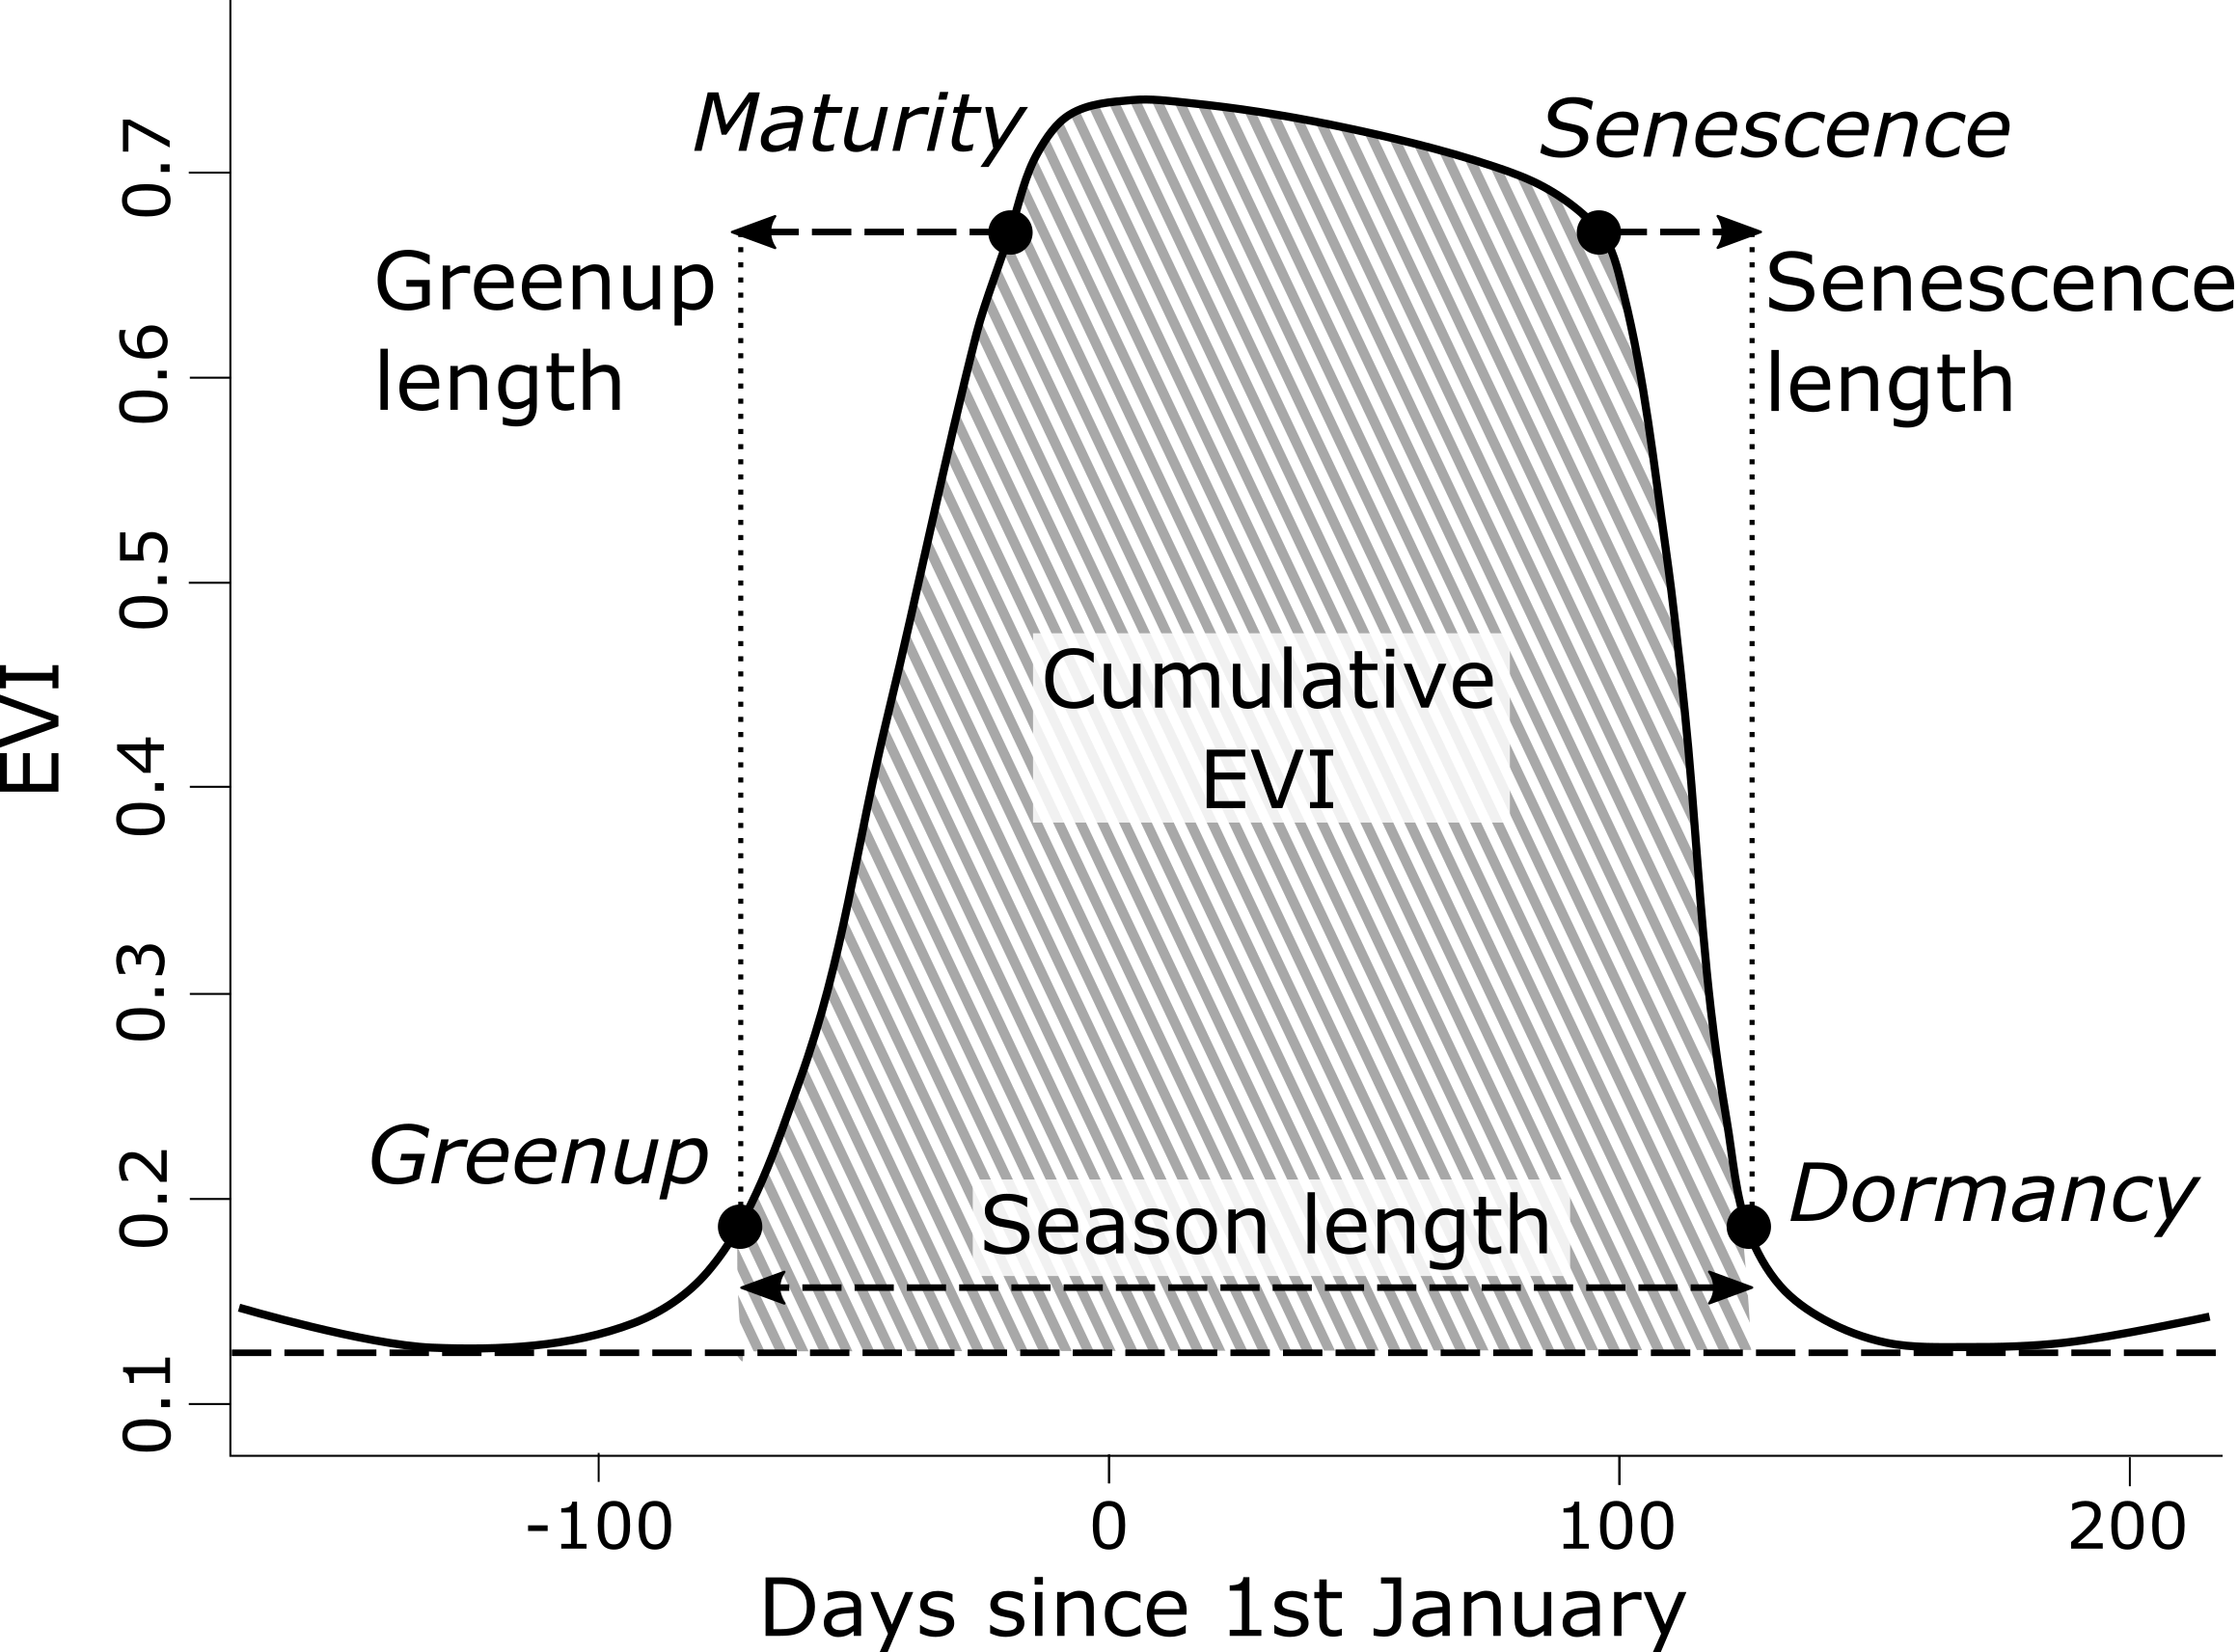
\includegraphics[width=0.8\textwidth]{ts_illus}
	\caption{Schematic diagram of hypothetical splined NBAR-EVI2 time series
		(black curve), from which metrics provided by the MCD12Q2 product are
		derived (black circles). Cumulative EVI indicates the shaded area under the EVI
		curve for a given growing season, bounded by the ``Greenup'' and ``Dormancy''
		dates. The blue curve shows a hypothetical splined 10 day rolling total
		rainfall time series, derived from the GPM IMERG product. Blue circles indicate
		the start and end of the rainy season as defined by our algorithm. Dashed black
		lines indicate the derived phenological metrics used in this study. In this
		hypothetical example, ``Greenup'' occurs in advance of the start of the rainy
		season, and ``Dormancy'' occurs after the end of the rainy season, reflecting
		the condition of 72.7\% (8451/11625) of the yearly data in our dataset. In
		26.7\% (3106/11625) of cases, senescence occurred after the end of the rainy
		season, but green-up occurred after the start of the rainy season. Adapted from
		\citep{Gray2022}.}
	\label{ts_illus}
\end{figure}

\subsubsection{Statistical modelling}

We used multivariate linear mixed effects models to investigate the effect of
tree species diversity, species composition, and woodland structure on each of
the six phenological metrics. We defined a maximal model structure including
the explanatory variables of species diversity, mean tree stem diameter, and
relative abundance of Detarioideae species, alongside climatic variables shown
by previous studies to strongly influence patterns of foliage production and
senescence: precipitation and cumulative temperature. For models of growing
season length and cumulative EVI we used total cumulative rainy season
precipitation and total cumulative rainy season temperature; for pre-rain
green-up and length of green-up period we used pre-green-up precipitation and
cumulative temperature; for senescence lag and length of senescence period we
used pre-senescence precipitation and cumulative temperature. We included
interaction terms for species diversity and mean stem diameter with vegetation
type, to test whether variation in community composition among vegetation types
mediated the effect of these variables on land surface phenology. All models
included a random intercept term for site to account for yearly repeated
measurements of site land surface phenology. We used the \texttt{dredge}
function from the \texttt{MuMIn} R package to determine which combination of
explanatory variables and their interactions best explained each phenological
metric. \texttt{dredge} produces a suite of models containing all possible
combinations of explanatory variables and their defined interactions. Candidate
models were compared using the model log-likelihood, AIC (Akaike Information
Criteria), conditional R\textsuperscript{2}. Where similar models were within
two AIC points of each other, the model with fewer terms was chosen as the best
model, to maximise model parsimony. Explanatory variables in each model were
standardised to Z-scores prior to modelling to allow comparison of slope
coefficients within a given model.

We assessed standardised effect sizes for explanatory variables in each best
model, re-estimated using Maximum Likelihood, to determine the magnitude and
direction of their effect on each phenological metric. For each explanatory
variable we calculated the 95\% confidence interval of the effect size as
1.96$\times{}$ the standard error of the parameter estimate \citep{Zuur2010}.
To investigate variation in the role of species diversity and woodland
structure on phenological metrics among vegetation types, we estimated marginal
means for these explanatory variables for each of the vegetation types, if they
appeared in the best model. We estimated marginal means using the
\texttt{ggeffects} package in R. Estimating marginal means entails generating
model predictions across values of a focal variable, while holding non-focal
variables constant at their reference value. We estimated marginal means across
the full range of each predictor in our dataset (species richness:
\richPredMin{}-\richPredMax{}, mean stem diameter: \dqmPredMin{}-\dqmPredMax{}
cm).

To identify significant variation in land surface phenology among vegetation
types we conducted a MANOVA using site median phenological metrics across the
study period as response variables, followed by post-hoc Tukey's tests between
each pairwise combination of vegetation types per phenological metric, to test
whether vegetation types differed significantly in their land surface
phenology. All statistical analyses were conducted in R version 4.0.2
\citep{R2020}.

\section{Results}

Multivariate linear mixed effects models effectively explained pre-rain
green-up (R\textsuperscript{2}\textsubscript{m}=\glagRm{},
R\textsuperscript{2}\textsubscript{c}=\glagRc{}), cumulative EVI
(R\textsuperscript{2}\textsubscript{m}=\cumviRm{},
R\textsuperscript{2}\textsubscript{c}=\cumviRc{}), season length
(R\textsuperscript{2}\textsubscript{m}=\lengthRm{},
R\textsuperscript{2}\textsubscript{c}=\lengthRc{}) and green-up length
(R\textsuperscript{2}\textsubscript{m}=\grateRm{},
R\textsuperscript{2}\textsubscript{c}=\grateRc{}), while senescence length
(R\textsuperscript{2}\textsubscript{m}=\srateRm{},
R\textsuperscript{2}\textsubscript{c}=\srateRc{}) and senescence lag
(R\textsuperscript{2}\textsubscript{m}=\slagRm{},
R\textsuperscript{2}\textsubscript{c}=\slagRc{}), were poorly constrained even
in the best models, according to the model selection procedure. Fixed effects
explained a large proportion of the total variance explained in models for
pre-rain green-up, season length and green-up length, while the random effect
of site explained most of the variance in cumulative EVI.

We compared standardised slope coefficients of explanatory variables within the
best model for each phenological metric to determine the strength and direction
of their influence (\autoref{mod_slopes}, \autoref{dredge}). Tree species
diversity exhibited strong positive effects on season length
(H\textsubscript{1}) and pre-rain green-up (H\textsubscript{2}). In contrast,
species diversity exhibited a strong negative effect on senescence lag, though
this model explained little of the total variance in senescence lag. Average
tree size, measured by the quadratic mean of stem DBH per site, was a
significant predictor of pre-rain green-up and green-up length
(H\textsubscript{3}). The relative basal area abundance of Detarioideae species
was a significant predictor of pre-rain green-up, season length and senescence
lag (H\textsubscript{4}). 

The slope of relationships between diversity and structural metrics and
phenological metrics varied little among vegetation types (\autoref{mod_marg}).
The strong positive effect of species diversity on season length and pre-rain
green-up was shared among all vegetation types. The effect of mean stem
diameter on pre-rain green-up and green-up length varied markedly by vegetation
type, with a negligible effect of this variable on green-up patterns in
Cryptosepalum miombo and Julbernardia miombo, but stronger positive effects in
Uapaca miombo and Combretaceae woodland.
 
A MANOVA using site median values for each phenological metric, showed a
significant difference among vegetation types (\phenManova{}). Combretaceae
woodlands had a significantly shorter growing season length than the other
vegetation types, along with significantly shorter periods of green-up
(\autoref{boxplots}). The majority of plots, regardless of vegetation type,
exhibited some degree of pre-rain green-up, with some inter-annual variation.
Across all sites, the mean lag between green-up and the onset of seasonal rains
was \greenLagMean{} days ($\pm{}$1 standard deviation).

\begin{figure}[H]
\centering
	\includegraphics[width=\textwidth]{mod_slopes.pdf}
	\caption{Standardised slope coefficients for the best model of each
		phenological metric. Slope estimates are $\pm$95\% confidence interval.
		Slope estimates where the interval does not overlap zero are considered to be
		significant effects and are marked by asterisks.}
	\label{mod_slopes}
\end{figure}

\begin{figure}[H]
\centering
	\includegraphics[width=\textwidth]{mod_marg.pdf}
	\caption{Marginal effects of tree species diversity on each of the
		phenological metrics, from the best-fitting multivariate linear model, for
		each vegetation type. Dotted lines represent 95\% confidence intervals for each
		vegetation type. Units of `d' are number of days.}
	\label{mod_marg}
\end{figure}

\begin{figure}[H]
\centering
	\includegraphics[width=0.8\textwidth]{boxplots.pdf}
	\caption{Boxplots of the six phenological metrics used in the study,
		grouped by vegetation type. Letters not shared among vegetation types
		denote that these vegetations types were identified as significantly different
		by post-hoc Tukey's HSD tests derived from the MANOVA of phenological metrics
		by vegetation type. Units of `d' are number of days.}
	\label{boxplots}
\end{figure}

\section{Discussion}

We have demonstrated clear and measurable effects of tree species diversity,
composition and structure on various metrics of land surface phenology in
deciduous woodlands across Zambia. Tree species diversity was associated with a
longer growing season and with earlier pre-rain green-up across woodland
compositional types. We also find that sites with a greater basal area
abundance of trees from the Detarioideae (subfamily of Fabaceae) tend to
green-up earlier in advance of the rainy season. Together, these results imply
that at least some of this species diversity effect may be driven by the
increased likelihood of containing species able to green-up earlier, i.e. a
mass-ratio effect \citep{Grime1996}. Our study lends support for a general
positive effect of tree species diversity on primary productivity in southern
African deciduous woodlands. 

Our finding that species diversity was associated with earlier pre-rain
green-up suggests that diverse woodlands may be more resilient to temporal
variations in the onset of seasonal rainfall. The phenomenon of pre-rain
green-up provides early forage for herbivores \citep{Morellato2016}, and
provides facilitative effects such as cover and hydraulic lift which benefit
understorey plants \citep{Domec2010, Yu2015}. Our results highlight the role of
tree species diversity as a driver of key ecosystem processes, affecting
ecosystem structure, the wildlife provisioning role, and Gross Primary
Productivity (GPP) \citep{Richardson2009}. 

The basal area abundance of Detarioideae species had a positive effect on
pre-rain green-up. Given their tendency to create deep root networks
\citep{Zhou2020}, and their conservative leaf economic spectrum traits, which
increase the resilience of leaves to environmental stresses such as cold and
drought \citep{Wigley2016}, we suggest that compared to other co-occurring
taxonomic groups, Detarioideae species are better equipped to green-up before
seasonal rainfall begins. While at present this ability to green-up prior to
the rainy season provides a competitive advantage to Detarioideae species, it
is unclear whether this behaviour might also lead to increased mortality
through hydraulic failure under a changing climate, where the date of onset of
the rainy season is predicted to become more erratic \citep{Vinya2018}.
Ultimately, it is not well defined how close these dominant species are to the
edge of their climatic niche \citep{Jinga2019}. Given the dominance of
Detarioideae species in deciduous woodlands across southern Africa, increased
mortality of this group may affect the future structure and composition of
these woodlands, with consequences for patterns of land surface phenology and
therefore woody productivity.

Environmental variables had consistently strong effects on phenological
metrics, and confirm previous research. Greater rainfall within the rainy
season led to a longer growing season and greater cumulative EVI, matching our
expectations that increased water availability allows for greater foliage
production and builds groundwater reserves allowing for a longer growing
season. Greater rainfall in the 30 days leading up to the start of the growing
season was associated with later green-up with respect to the timing of the
onset of the rainy season. We suggest this may be the result of large amounts
of rainfall kick-starting foliage production in the absence of a pre-rain
green-up effect in some plots, and may represent cases where grasses drive the
start of growing season land surface phenology signal. Hotter days led to
shorter periods of senescence and green-up. In the case of green-up length,
this effect may imply an increasing temperature trigger on foliage production,
as is seen in temperate woodland ecosystems \citep{Flynn2018}. In the case of
senescence, this effect may be due to hot days causing wilting of old leaves
under reduced water availability at the end of the rainy season
\citep{Warren2011, Marin2019}. This study provides a glimpse into how extreme
climatic events, particularly heat and drought events, could strongly affect
leaf phenology in the future under a changing climate in southern Africa
\citep{Naumann2018}. Increased temperature and decreased precipitation were
both strongly associated with decreased growing season length, and reduced
pre-rain green-up. Future studies would be well-placed to explore further how
climate extremes affect land surface phenology, ideally in combination with
measurements of composition and structure, which we expect might mediate the
effect of climate extremes.

The lag between the end of the growing season and the end of the rainy season
was negatively influenced by tree mean stem diameter, though our model had low
explanatory power. \citet{Cho2017} similarly found that tree cover, measured by
MODIS Leaf Area Index (LAI) data, had a significant negative effect on
senescence rates in woodlands in South Africa, which have similar climatic
conditions to the sites in our study. In most woodlands, including sparse
savannas, while the onset of the growing season is often driven by tree
photosynthetic activity \citep{Ryan2017, Archibald2007, Chidumayo2001}, which
may precede the onset of precipitation, the end of the growing season is
conversely driven by the understorey grass layer \citep{Cho2017, Guan2014}.
Grass activity is more reactive to short-term changes in soil moisture than
tree activity, and may oscillate within the senescence period
\citep{Archibald2007}. This may explain the lack of a strong precipitation or
diversity signal for senescence lag and length of the senescence period in our
models.

% Why didn't we get strong models for length of greening and senescence periods?
Our best models predicting the length of the green-up and senescence period did
not explain much of the variance in these phenological metrics. Length of the
green-up period varied significantly among vegetation types, implying that the
particular combination of species and the synchrony of their phenological
strategy might be the determining factor for this phenological metric. Though
more work must be done to explore this further. As mentioned above, short term
oscillations in soil moisture and the condition of ground cover vegetation may
be responsible for driving the length of the senescence period, hence the wide
variability of this phenological metric and the poor fit of our statistical
models. Indeed, most of the variance explained by our model of senescence
length and senescence lag came from the random effect of site, implying some
unmeasured inter-site variation, possibly in community composition. 

% Good para, no changes
It is striking that the fixed effects in our models were unable to explain
variation in the length of the senescence period or the lag between the end of
the growing season and the end of the rainy season. The random effect of site
accounted for most of the variance explained by these models, implying high
variation among sites as compared to within sites. This suggests that there are
some unmeasured environmental or biotic factors at play in determining
senescence in these systems. 

Other studies, both globally and within southern African woodlands, have
largely ignored patterns of senescence, instead focussing on patterns of
green-up \citep{Gallinat2015}. Most commonly, these studies simply correlate
the decline of rainfall with senescence \citep{Stevens2016, Guan2014}, but our
best model suggests that temperature is a stronger determinant of the end of
the growing season than precipitation. We suggest that hotter days in the
period leading up to the start of the senescence period might accelerate
senescence due to wilting, resulting in a shorter senescence period length. In
temperate ecosystems, which experience autumn senescence, lower night time
temperatures have been shown to increase the rate of senescence and thus
decrease senescence period length \citep{Michelson2017, Escamilla2020}. In
these water-limited and hot systems however, it seems hotter temperatures are
the main driver. Similarly, hotter days prior to senescence appear to advance
the onset of senescence with respect to the end of the rainy season, which may
also be caused by wilting as rainfall starts to decrease. These suggestions
however, must be considered in the context that the fixed effects in our models
did not account for much of the variation in senescence period length or
senescence lag.

% Good para, no changes
Alternatively, \citet{Zani2020} suggests that in resource-limited environments,
senescence times may largely be set by the preceding photosynthetic activity
and sink-limitations on growth. For example, limited nutrient supply may
prohibit photosynthesis late in the season if the preceding photosynthetic
activity has depleted that supply. \citet{Reich1992} suggested that there are
many direct constraints on leaf life-span such as drought and herbivory,
especially in the seasonally dry tropics, which would lead to timing of
senescence being set largely by the time of bud-burst. Our study indirectly
corroborates this theory, with the finding of a moderate positive correlation
between pre-rain green-up and senescence lag across all vegetation types,
indicating that later green-up allows later senescence (\autoref{phen_bivar}).

We found positive effects of mean tree size (site quadratic mean diameter) on
pre-rain green-up and green-up length, but negative effects on senescence lag.
We suggest that the increased rooting depth of large trees, allows them to
access deep ground-water reserves, conferring resilience to inter-annual
variation in patterns of seasonal rainfall \citep{Holdo2017}. This result
provides a possible mechanism by which certain groups of species, like those of
the subfamily Detarioideae, are able to drive earlier pre-rain green-up, as
they generally grow to larger sizes. Our results suggest a mass-ratio effect in
the pre-rain green-up of Zambian deciduous woodlands \citep{Grime1998}, whereby
dominant functional groups of trees which grow to large sizes are able to
green-up in advance of seasonal rains, drive longer growing seasons, and
overall drive greater productivity.

% Good para, no changes
Our finding that species diversity increases season length and cumulative EVI
in seasonally dry tropical woodlands provides an example of a mechanism by
which species diversity increases ecosystem function, a pattern observed
previously in other studies of southern African woodlands \citep{Godlee2021,
McNicol2018, Shirima2015}, and globally in other biomes \citep{Plas2019,
Tilman2014}. Our findings provide earth surface system modellers with a means
to better understand how changes in the inter-related variables of species
diversity, composition and structure affect land surface phenology.
Incorporating predictions of biotic composition and its change over time into
earth system models has been limited until recently for two main reasons
\citep{Ahlstrom2015, Bodegom2011}. Firstly, there are large uncertainties in
the effects of biodiversity on ecosystem function, e.g. gross primary
productivity (GPP). Secondly, until recently there has been a major paucity of
ground data on community composition. Our study comes at a pertinent time when
plot-based vegetation monitoring networks have become sufficiently widespread
\citep{ForestPlotsnet2021, SEOSAW2020}, and remotely sensed proxies of
diversity in forested ecosystems are becoming sophisticated enough
\citep{Schneider2017, Cavendar2020} to be of real use to earth system
modellers. Our study provides a link by demonstrating a strong relationship
between species diversity and land surface phenology, particularly growing
season length, which is itself closely correlated with GPP
\citep{Sjostrom2011}. 

\section{Conclusion}

We explored how tree species diversity, composition and structure of deciduous
woodlands influence land surface phenology across Zambia. We showed that
species diversity drives longer growing seasons and promotes earlier pre-rain
green-up across all woodland compositional types studied here. The abundance of
Detarioideae species (subfamily of Fabaceae) had a consistent positive effect
on pre-rain green-up and over-all growing season length, supporting suggestions
from previous studies of their keystone role in driving pre-rain green-up in
southern African miombo woodlands. We found an effect of mean tree size on land
surface phenology, and it is likely that larger potential tree size in
Detarioideae species is one trait facilitating pre-rain green-up. Finally, we
have demonstrated variation in phenological patterns among woodland
compositional types within Zambia that are not commonly distinguished in
classifications of woodland types in the region. 

Our results lend further support to an already well established corpus of study
on the positive effect of species diversity on ecosystem function.
Additionally, our results provide evidence for earth-system modellers,
demonstrating the importance of community composition, structure and diversity
in determining patterns of land surface phenology. As reliable data on plant
community composition and structure becomes available across larger spatial
scales and at higher spatial resolution, we hope that these data can be
included in models of land-atmosphere mass and energy exchange to improve their
predictive power.

\printbibliography

\section{Supplementary Material}
\beginsupplement

\begin{figure}[H]
\centering
	\includegraphics[width=\textwidth]{phen_bivar}
	\caption{Scatter plots showing pairwise comparisons of the six phenological
		metrics used in this study, extracted from the MODIS MCD12Q2 product
		\citep{MCD12Q2}. Points represent study sites and are coloured by vegetation
		type. Linear regression line of best fit for all sites is shown as a black
		line, while linear regressions are shown for each vegetation type as coloured
		lines. Non-significant linear regression fits (p<0.05) have dashed lines. The
		units of `d' are the number of days.}
	\label{phen_bivar}
\end{figure}

\setlength{\tabcolsep}{1pt} % Default table column sep width 
\begin{landscape}
\input{out/dredge_adj.tex}
\end{landscape}
\setlength{\tabcolsep}{4pt} % Default table column sep width 

\end{document}

